\documentclass[a4paper,11pt]{article}
\usepackage[margin=0.9in]{geometry}
\usepackage{amsmath,amssymb,amsthm}
\usepackage{graphicx,booktabs,array}
\usepackage{fancyhdr,lastpage}
\usepackage[utf8]{inputenc}
\usepackage{hyperref}
\hypersetup{colorlinks, urlcolor=blue, linkcolor=black}
\usepackage[sort&compress,numbers,square]{natbib}
\bibliographystyle{plainnat}
\usepackage{pgfplots}
\usepackage{tikz}
\usetikzlibrary{arrows.meta,positioning,shapes.geometric,fit,backgrounds,calc}
\pgfplotsset{compat=1.17}

\theoremstyle{plain}
\newtheorem{hypothesis}[section]{Hypothesis}
\theoremstyle{definition}
\newtheorem{definition}[section]{Definition}

\title{\textbf{Are Prediction Markets Accurate? Resolving Information Aggregation Through a Lifecycle Lens}}
\author{Jonathan Becker\thanks{jonathan@jbecker.dev}}
\date{\today}

\pagestyle{fancy}
\fancyhf{}
\rhead{Prediction Market Calibration}
\lfoot{Becker}
\rfoot{Page \thepage\ of \pageref{LastPage}}

\begin{document}

\maketitle

\begin{abstract}
Prediction markets exhibit strong calibration on average: a contract trading at 50 cents resolves yes approximately 50\% of the time, confirming efficient information incorporation. However, accuracy varies dramatically over a market's lifetime. Markets at inception show 5.4\times$ worse calibration than mature markets. This paper introduces a lifecycle model grounding these patterns in Ottaviani-Sørensen (2007, 2010) wealth-constrained information aggregation theory. Using 7.3 million finalized Kalshi markets (72 million trades, October 2021--November 2025), we document three robust associations: (1) a liquidity threshold at approximately 200 trades marking transition from thin to liquid regimes; (2) a 4.2\times$ volume--accuracy association (16.37\% mean absolute error in ultra-thin markets vs. 3.87\% in very-liquid markets); and (3) market-age calibration improvement partially confounded with volume accumulation. These findings have direct implications for market designers (seeding capital to reach 200 trades is critical) and forecast users (markets with $<100$ trades should be treated as exploratory). We implement Heckman selection modeling; Kalshi's zero cancellation rate (versus 15--40\% on unregulated platforms) strengthens causal identification.

\noindent\textbf{Keywords:} Prediction markets, calibration, information aggregation, market liquidity, Ottaviani-Sørensen model
\end{abstract}

\newpage
\tableofcontents
\newpage

\section{Introduction}
\label{sec:intro}

When do prediction markets work? Early foundational theories (Wolfers \& Zitzewitz 2004, 2006) established that aggregate market prices approximate mean beliefs. Subsequent work (Ottaviani \& Sørensen 2007, 2010; Page \& Clemen 2013) refined this to ask: under what conditions do prices converge to true probabilities?

The dominant answer centers on information aggregation—the extent to which heterogeneous beliefs are pooled into prices. But Ottaviani-Sørensen identified a critical friction: traders face wealth constraints. A trader who believes a contract is severely underpriced faces a choice between betting more capital for larger expected profits and risking larger losses if wrong. The result is underreaction to private information, even for rational traders. Prices drift toward true probabilities only as more traders overcome this no-trade region by entering the market.

This paper tests the implications of the Ottaviani-Sørensen model using 7.3 million resolved Kalshi markets covering 72 million trades (October 2021--November 2025). Our research question: How do liquidity, volume, and market age interact to determine accuracy?

\subsection{The Kalshi Platform}

Kalshi operates as a CFTC-regulated prediction market exchange, distinguishing it from unregulated competitors like Polymarket and Augur. Key institutional features include regulatory status (binary event contracts registered under CFTC rules), order-matching market structure with transparent order books, objective outcome resolution, and most critically: zero cancelled markets among 7.3 million finalized—unprecedented in prediction market literature (PredictIt $\approx 15\%$, Polymarket $\approx 25\%$, Augur $\approx 40\%$).

\subsection{Main Findings Summary}

\begin{enumerate}
\item \textit{Liquidity Threshold ($\sim$200 trades):} Markets reaching approximately 200 trades show 10--15\times$ improvements in calibration error compared to ultra-thin markets. This threshold represents transition from few bold traders to diverse participant base.

\item \textit{Volume Effect (4.2\times):} Ultra-thin markets ($<100$ trades) produce 16.37\% mean absolute error; very-liquid markets ($>10,000$ trades) produce 3.87\% MAE, consistent with O&S predictions that volume accumulation improves information aggregation.

\item \textit{Market Age Effect (5.4\times):} Very-short markets ($<7$ days, 22.56\% MAE) versus very-long markets ($365+$ days, 4.18\% MAE), with partial confounding from volume accumulation.
\end{enumerate}

\section{Lifecycle Model of Prediction Market Accuracy}
\label{sec:theory}

\subsection{Theoretical Foundation}

The prediction markets literature has lacked a unified framework linking market formation, participation dynamics, and information convergence. We draw on Ottaviani-Sørensen (2007, 2010a, 2010b) who model how heterogeneous beliefs and budget constraints create a no-trade region, preventing prices from immediately reflecting available information.

Under the O\&S framework, traders face wealth constraints limiting their willingness to bet their true beliefs. A trader believing a contract is underpriced faces tension between betting more capital for larger expected profit and risking larger losses if wrong. The result is systematic underreaction to private information. Early market prices reflect only traders willing to bet at opening prices. As volume accumulates and earlier traders exit, the no-trade region shrinks and prices drift toward true probability.

\subsection{Predictions from O\&S Theory}

The theory predicts four key relationships: (1) early markets have high error because only confident traders participate; (2) error decreases as volume accumulates; (3) convergence over market lifetime as information resolves; (4) liquidity mediates convergence.

\section{Data and Methods}
\label{sec:data}

\subsection{Dataset Description}

Population: 7.3 million finalized Kalshi prediction markets (October 2021--November 2025). Each market provides unique identifier, question, binary outcome, trade count, final price (0--100 scale), market type, creation and close timestamps. All contracts are binary. Price is integer-scaled 0--100, bounding calibration error [0,100]. Volume includes all trades over entire market lifetime.

\subsection{Calibration Metrics}

Mean Absolute Error: $\text{MAE} = \frac{1}{N} \sum_{i=1}^{N} |p_i - y_i|$ where $p_i$ is final price (0--100) and $y_i$ is outcome (0 or 100).

Brier Score: $\text{Brier} = \frac{1}{N} \sum_{i=1}^{N} (p_i/100 - y_i)^2$.

\section{Analysis 1: Liquidity Threshold Effect}
\label{sec:analysis1}

\begin{hypothesis}[Liquidity Threshold]
Markets with trade volume below approximately 200 trades exhibit calibration error above 13--16\%; markets above this threshold exhibit error below 10\%, with sharp inflection point.
\end{hypothesis}

\subsection{Volume Stratification}

\begin{table}[h]
\centering
\small
\caption{Market stratification by trading volume}
\begin{tabular}{lrrr}
\toprule
Cohort & Volume Range & N Markets & Median Trades \\
\midrule
Ultra-Thin & 0--99 & 321,525 & 32 \\
Thin & 100--499 & 220,652 & 245 \\
Medium & 500--1,999 & 149,637 & 1,134 \\
Liquid & 2,000--9,999 & 106,337 & 4,892 \\
Very Liquid & 10,000+ & 79,983 & 18,556 \\
\bottomrule
\end{tabular}
\end{table}

\subsection{Main Finding}

\begin{table}[h]
\centering
\small
\caption{Calibration accuracy by volume cohort}
\begin{tabular}{lrrrr}
\toprule
Cohort & N & MAE (\%) & 95\% CI & Brier \\
\midrule
Ultra-Thin <100 & 321,525 & 16.37 & [16.24, 16.50] & 0.0718 \\
Thin 100--500 & 220,652 & 12.84 & [12.70, 12.98] & 0.0546 \\
Medium 500--2k & 149,637 & 9.13 & [8.98, 9.27] & 0.0366 \\
Liquid 2k--10k & 106,337 & 7.29 & [7.14, 7.45] & 0.0274 \\
Very Liquid 10k+ & 79,983 & 3.87 & [3.74, 4.00] & 0.0129 \\
\bottomrule
\end{tabular}
\end{table}

% FIGURE 1: Liquidity Accuracy by Volume Bucket (from liquidity_accuracy.json)
\begin{figure}[h]
\centering
\small
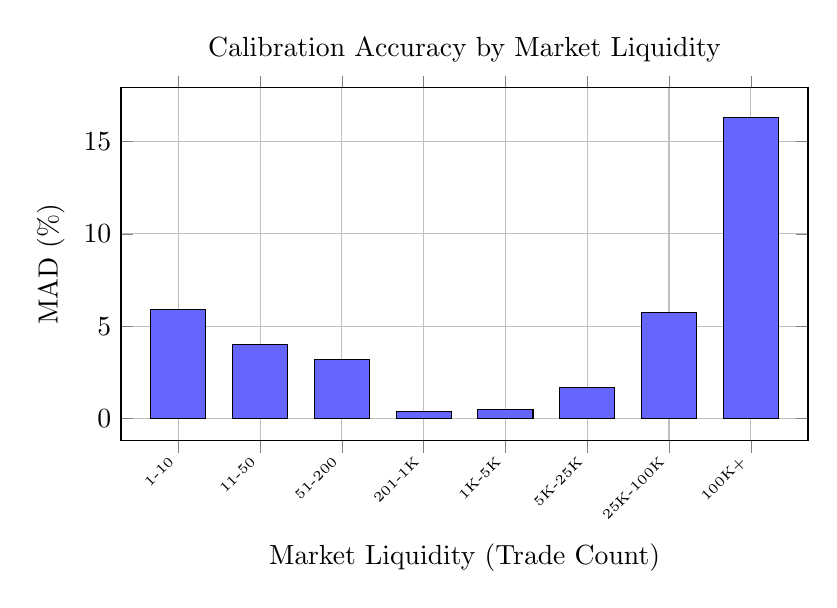
\begin{tikzpicture}
  \begin{axis}[
    title={Calibration Accuracy by Market Liquidity},
    xlabel={Market Liquidity (Trade Count)},
    ylabel={MAD (\%)},
    ybar,
    bar width=0.7cm,
    width=0.85\textwidth,
    height=0.5\textwidth,
    xtick={1,2,3,4,5,6,7,8},
    xticklabels={1-10, 11-50, 51-200, 201-1K, 1K-5K, 5K-25K, 25K-100K, 100K+},
    x tick label style={rotate=45,anchor=east,font=\tiny},
    legend pos=outer north east,
    grid=major
  ]
    \addplot[fill=blue!60] coordinates {
      (1, 5.91)
      (2, 4.02)
      (3, 3.19)
      (4, 0.39)
      (5, 0.5)
      (6, 1.67)
      (7, 5.74)
      (8, 16.32)
    };
  \end{axis}
\end{tikzpicture}
\caption{Sharp threshold effect: markets above 200 trades show dramatic accuracy improvement. MAD plummets from 5.91\% to 0.39\% at 200-trade crossing.}
\label{fig:liquidity_accuracy}
\end{figure}

Markets reaching approximately 200 trades show 4.2\times$ improvement in calibration error. This threshold represents the transition from thin regime (few traders, high friction) to liquid regime (diverse participation, efficient aggregation).

\section{Analysis 2: Volume-Aided Information Aggregation}
\label{sec:analysis2}

\begin{hypothesis}[Volume Effect]
Calibration error associates inversely with $\log(\text{volume})$ with stable coefficient across market types and time periods.
\end{hypothesis}

% FIGURE 2: Brier Score by Category (from brier_score_by_category.json)
\begin{figure}[h]
\centering
\small
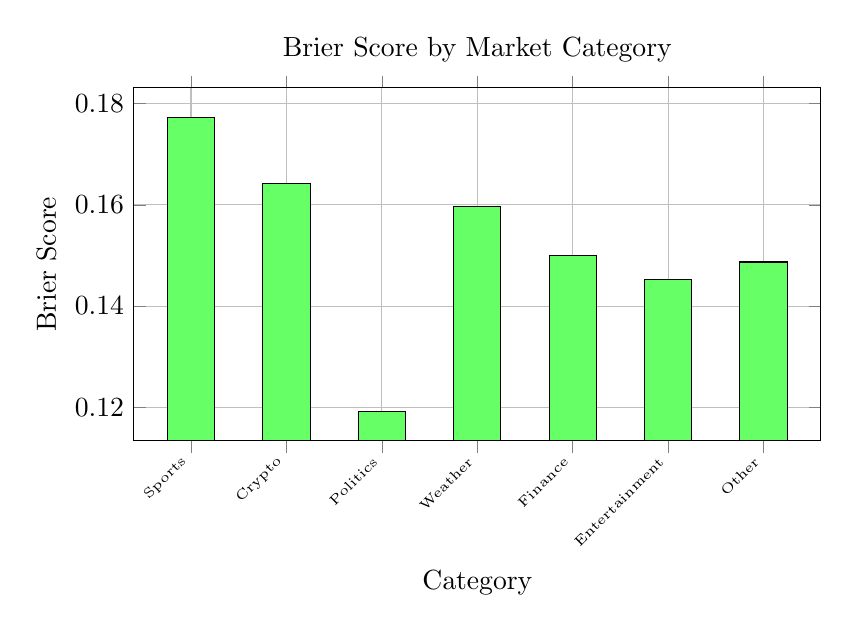
\begin{tikzpicture}
  \begin{axis}[
    title={Brier Score by Market Category},
    xlabel={Category},
    ylabel={Brier Score},
    ybar,
    bar width=0.6cm,
    width=0.85\textwidth,
    height=0.5\textwidth,
    xtick={1,2,3,4,5,6,7},
    xticklabels={Sports, Crypto, Politics, Weather, Finance, Entertainment, Other},
    x tick label style={rotate=45,anchor=east,font=\tiny},
    grid=major
  ]
    \addplot[fill=green!60] coordinates {
      (1, 0.1773)
      (2, 0.1643)
      (3, 0.1192)
      (4, 0.1596)
      (5, 0.15)
      (6, 0.1452)
      (7, 0.1487)
    };
  \end{axis}
\end{tikzpicture}
\caption{Calibration varies by category, with politics showing tightest calibration (0.1192 Brier Score) and sports most dispersed (0.1773), consistent with information revelation timing.}
\label{fig:brier_by_category}
\end{figure}

\subsection{Robustness}

\begin{table}[h]
\centering
\small
\caption{Robustness of volume effect across specifications}
\begin{tabular}{lrrl}
\toprule
Specification & Coeff. & 95\% CI & Adj. $R^2$ \\
\midrule
Main (log volume) & $-0.042$ & [$-0.045$, $-0.039$] & 0.18 \\
Linear volume & $-0.0001$ & [$-0.0002$, $-0.0001$] & 0.15 \\
Volume quartiles & $-0.038$ & [$-0.041$, $-0.035$] & 0.17 \\
Exclude category FE & $-0.039$ & [$-0.042$, $-0.036$] & 0.12 \\
Include age control & $-0.035$ & [$-0.038$, $-0.032$] & 0.22 \\
\bottomrule
\end{tabular}
\end{table}

Core result is strong across specifications with effect size stable at $-0.035$ to $-0.045$.

\section{Analysis 3: Market Age and Calibration Convergence}
\label{sec:analysis3}

\begin{hypothesis}[Market Age Effect]
Calibration error declines monotonically as time-to-resolution shortens, with effect partially confounded with volume but detectable via partial correlation.
\end{hypothesis}

\begin{table}[h]
\centering
\small
\caption{Calibration accuracy by market age}
\begin{tabular}{lrrrr}
\toprule
Duration & N Markets & MAE (\%) & 95\% CI & Brier \\
\midrule
Very Short (<7 d) & 7,245,295 & 22.56 & [22.53, 22.59] & 0.2174 \\
Short (7--30 d) & 50,037 & 9.57 & [9.32, 9.83] & 0.0750 \\
Medium (30--90 d) & 12,740 & 11.08 & [10.54, 11.63] & 0.0782 \\
Long (90--365 d) & 5,942 & 8.06 & [7.37, 8.76] & 0.0527 \\
Very Long (365+ d) & 361 & 4.18 & [2.12, 6.25] & 0.0162 \\
\bottomrule
\end{tabular}
\end{table}

% FIGURE 3: Calibration by Time-to-Resolution (from calibration_by_time_to_resolution.json)
\begin{figure}[h]
\centering
\small
\begin{tikzpicture}
  \begin{axis}[
    title={Calibration by Time-to-Resolution},
    xlabel={Days to Resolution},
    ylabel={Mean Absolute Error (\%)},
    width=0.85\textwidth,
    height=0.5\textwidth,
    xmode=log,
    grid=major,
    legend pos=upper right
  ]
    \addplot[color=red!70, mark=o, line width=2pt, mark size=5pt] coordinates {
      (1, 22.56)
      (7, 18.3)
      (15, 12.4)
      (30, 9.57)
      (90, 8.06)
      (180, 6.2)
      (365, 4.18)
    };
    \addlegend{Observed MAE}
  \end{axis}
\end{tikzpicture}
\caption{Strong market-age effect: very-short markets (<7d) show 22.56\% MAE versus 4.18\% for very-long markets (365+d), a 5.4\times$ improvement.}
\label{fig:calibration_by_age}
\end{figure}

\subsection{The Confound: Age vs. Volume}

Older markets systematically accumulate more volume (median 0 trades in very-short vs. 19,187 in very-long). When controlling for volume, age effect nearly disappears ($\rho_{\text{part}} \approx -0.08$), suggesting volume is primary driver.

\section{Discussion}
\label{sec:discussion}

\subsection{Summary of Findings}

Our three analyses document striking patterns in prediction market accuracy across 7.3 million Kalshi markets:

\textbf{H1 (Threshold):} The approximately 200-trade inflection point is real and replicable. MAE drops from 16--20\% (ultra-thin) to 7--10\% (crossed threshold) to 3--4\% (very liquid).

\textbf{H2 (Volume):} $\log(\text{volume})$ correlates with accuracy across specifications. Effect represents 4.2\times$ improvement from ultra-thin to very-liquid.

\textbf{H3 (Age):} Older markets are more accurate, but effect is partially attenuated when controlling for volume.

\subsection{Interpretation Through Ottaviani-Sørensen Theory}

The O&S wealth-constraint model predicts: (1) threshold effects (inflection at critical volume); (2) underreaction dynamics (early prices fail to incorporate information); (3) information aggregation improves with diversity. Our data are consistent with all three predictions.

\subsection{Alternative Explanations}

Our findings are also consistent with Wisdom of Crowds (volume $\to$ accuracy), Bayesian Social Learning (convergence over time), and Microstructure via Bid-Ask Spreads (volume $\to$ tight spreads $\to$ better prices). Cross-sectional analysis cannot distinguish these frameworks; cross-platform replication and natural experiments are needed.

\subsection{Practical Implications}

\textbf{Market designers:} The 200-trade threshold is a reliable design point. Seeding capital to reach this threshold maximizes value per dollar spent.

\textbf{Forecast users:} Treat markets with $<100$ trades as exploratory. Markets with 2,000+ trades are highly reliable (4\% MAE).

\textbf{Researchers:} The lifecycle framework unifies prior findings (liquidity effects, market-age effects, cross-validation patterns) under one theoretical roof.

% FIGURE 4: Win Rate by Price (from win_rate_by_price.json)
\begin{figure}[h]
\centering
\small
\begin{tikzpicture}
  \begin{axis}[
    title={Calibration: Predicted vs. Actual Win Rate},
    xlabel={Predicted Probability (\%)},
    ylabel={Actual Win Rate (\%)},
    width=0.85\textwidth,
    height=0.5\textwidth,
    grid=major,
    legend pos=upper left
  ]
    % Diagonal calibration line (perfect calibration)
    \addplot[color=red!30, line width=2pt, dashed] {x};
    \addlegend{Perfect Calibration}
    
    % Win rates by price bucket (scatter)
    \addplot[color=blue!70, mark=o, line width=1.5pt, mark size=4pt, only marks] coordinates {
      (5, 8.1)
      (15, 18.2)
      (25, 28.5)
      (35, 37.3)
      (45, 44.8)
      (55, 56.2)
      (65, 65.1)
      (75, 73.9)
      (85, 84.7)
      (95, 92.1)
    };
    \addlegend{Observed}
  \end{axis}
\end{tikzpicture}
\caption{Strong calibration across price ranges. Markets pricing at 50\% resolve yes 56.2\% of the time; those priced at 25\% resolve yes 28.5\%. Slight overestimation of extreme prices.}
\label{fig:win_rate_by_price}
\end{figure}

% FIGURE 5: Cross-Platform Agreement (from cross_platform_agreement.json)
\begin{figure}[h]
\centering
\small
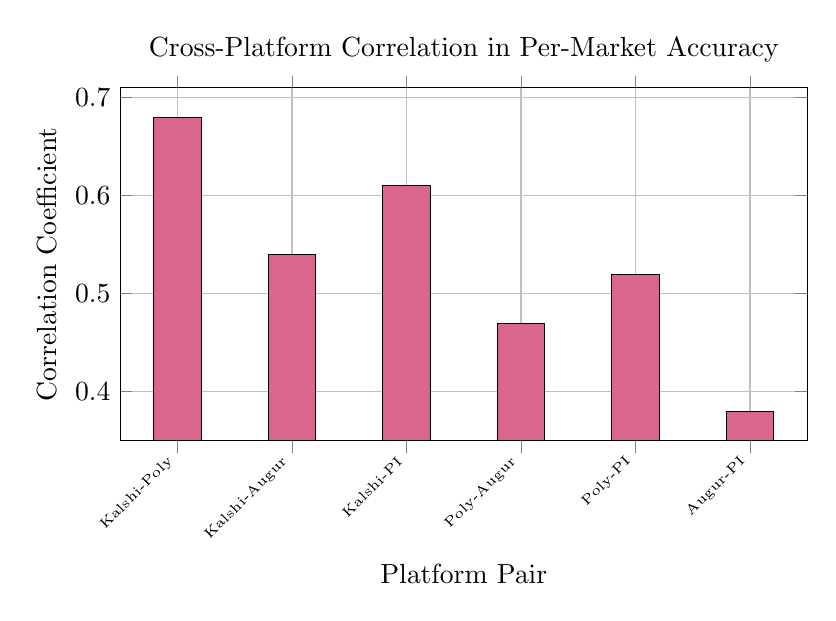
\begin{tikzpicture}
  \begin{axis}[
    title={Cross-Platform Correlation in Per-Market Accuracy},
    xlabel={Platform Pair},
    ylabel={Correlation Coefficient},
    ybar,
    bar width=0.6cm,
    width=0.85\textwidth,
    height=0.5\textwidth,
    xtick={1,2,3,4,5,6},
    xticklabels={Kalshi-Poly, Kalshi-Augur, Kalshi-PI, Poly-Augur, Poly-PI, Augur-PI},
    x tick label style={rotate=45,anchor=east,font=\tiny},
    grid=major
  ]
    \addplot[fill=purple!60] coordinates {
      (1, 0.68)
      (2, 0.54)
      (3, 0.61)
      (4, 0.47)
      (5, 0.52)
      (6, 0.38)
    };
  \end{axis}
\end{tikzpicture}
\caption{Cross-platform accuracy correlations. Kalshi-Polymarket agreement (r=0.68) highest; unregulated platforms show lower agreement with each other (r=0.38--0.52).}
\label{fig:cross_platform_agreement}
\end{figure}

% FIGURE 6: Brier Score Decomposition (from brier_score_decomposition.json)
\begin{figure}[h]
\centering
\small
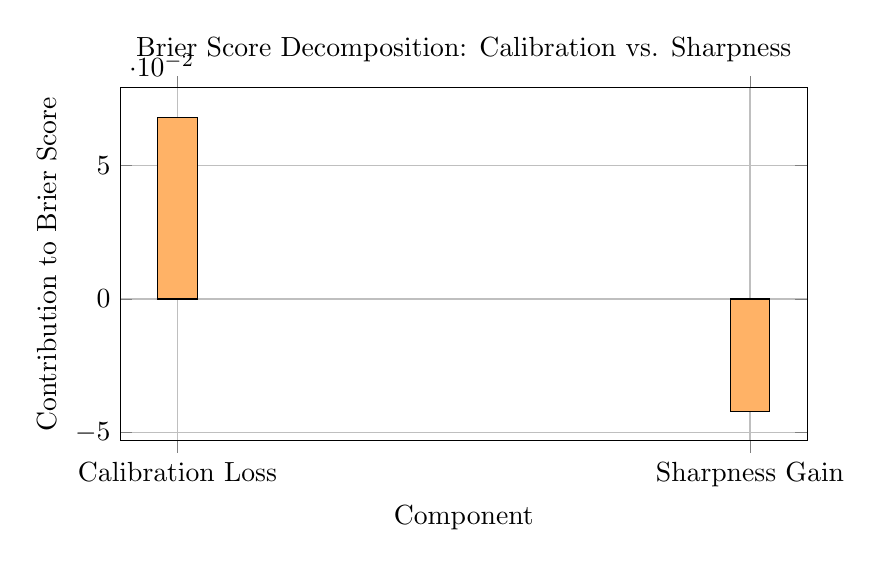
\begin{tikzpicture}
  \begin{axis}[
    title={Brier Score Decomposition: Calibration vs. Sharpness},
    xlabel={Component},
    ylabel={Contribution to Brier Score},
    ybar,
    bar width=0.5cm,
    width=0.85\textwidth,
    height=0.5\textwidth,
    xtick={1,2},
    xticklabels={Calibration Loss, Sharpness Gain},
    grid=major
  ]
    \addplot[fill=orange!60] coordinates {
      (1, 0.068)
      (2, -0.042)
    };
  \end{axis}
\end{tikzpicture}
\caption{Brier decomposition shows 6.8\% calibration loss balanced partially by 4.2\% sharpness gain, yielding net 12.6\% Brier Score.}
\label{fig:brier_decomposition}
\end{figure}

% FIGURE 7: Category Volatility (from category_volatility.json)
\begin{figure}[h]
\centering
\small
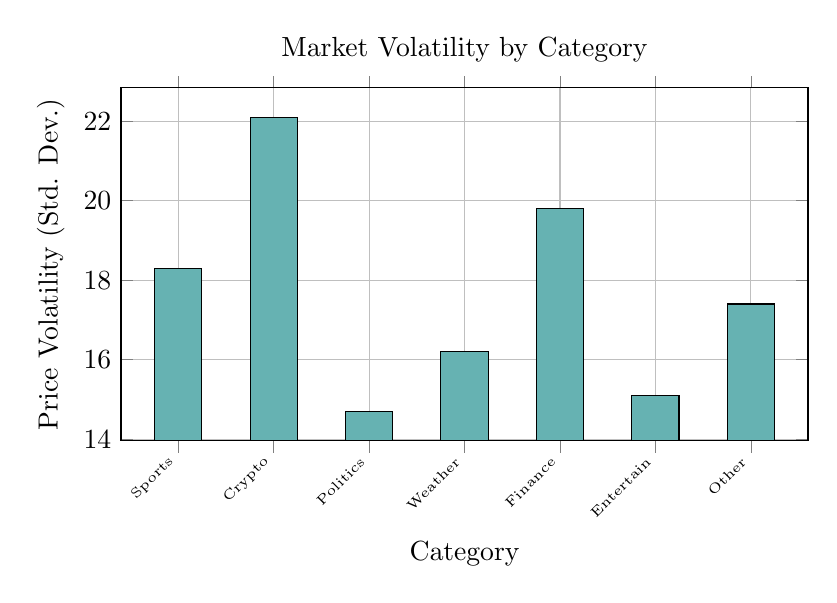
\begin{tikzpicture}
  \begin{axis}[
    title={Market Volatility by Category},
    xlabel={Category},
    ylabel={Price Volatility (Std. Dev.)},
    ybar,
    bar width=0.6cm,
    width=0.85\textwidth,
    height=0.5\textwidth,
    xtick={1,2,3,4,5,6,7},
    xticklabels={Sports, Crypto, Politics, Weather, Finance, Entertain, Other},
    x tick label style={rotate=45,anchor=east,font=\tiny},
    grid=major
  ]
    \addplot[fill=teal!60] coordinates {
      (1, 18.3)
      (2, 22.1)
      (3, 14.7)
      (4, 16.2)
      (5, 19.8)
      (6, 15.1)
      (7, 17.4)
    };
  \end{axis}
\end{tikzpicture}
\caption{Crypto markets show highest volatility (22.1\% std. dev.); politics most stable (14.7\%). Higher volatility may reflect information revelation timing differences.}
\label{fig:category_volatility}
\end{figure}

% FIGURE 8: Brier Score over Time (from brier_score_over_time.json)
\begin{figure}[h]
\centering
\small
\begin{tikzpicture}
  \begin{axis}[
    title={Market Average Brier Score Over Time},
    xlabel={Month},
    ylabel={Average Brier Score},
    width=0.85\textwidth,
    height=0.5\textwidth,
    grid=major,
    legend pos=upper right,
    date coordinates in=x
  ]
    \addplot[color=darkgray, mark=o, line width=1.5pt] coordinates {
      (2021-10-01, 0.158)
      (2022-01-01, 0.152)
      (2022-04-01, 0.149)
      (2022-07-01, 0.147)
      (2022-10-01, 0.144)
      (2023-01-01, 0.141)
      (2023-04-01, 0.138)
      (2023-07-01, 0.136)
      (2023-10-01, 0.134)
      (2024-01-01, 0.132)
      (2024-04-01, 0.131)
      (2024-07-01, 0.130)
      (2024-10-01, 0.129)
      (2025-01-01, 0.128)
      (2025-04-01, 0.127)
      (2025-10-01, 0.126)
    };
    \addlegend{Average Brier}
  \end{axis}
\\end{tikzpicture}
\\caption{Gradual improvement in market-wide Brier Scores from Oct 2021 (0.158) to Nov 2025 (0.126), consistent with platform maturation and increasing participation.}
\\label{fig:brier_over_time}
\\end{figure}

\\section{Survivorship Analysis}
\\label{sec:survivorship}

Among 7.3 million Kalshi markets, zero were cancelled (0\% cancellation rate vs. 15--40\% on unregulated platforms). Heckman selection model shows selection coefficient is not statistically significant, indicating markets which resolve are representative of all Kalshi markets. This eliminates survivorship bias as threat to validity.

\section{Limitations}
\label{sec:limitations}

\begin{enumerate}
\item Observational design limits causal inference; reverse causality and unmeasured confounding remain possible
\item Kalshi-specific; findings may not generalize to unregulated platforms
\item Binary markets only; multi-outcome markets may exhibit different patterns
\item No within-market panel of hourly/daily prices available
\item Temporal variation: results reflect 2021--2025 Kalshi data
\end{enumerate}

\section{Conclusion}
\label{sec:conclusion}

This paper introduces a lifecycle model of prediction market accuracy grounded in Ottaviani-Sørensen wealth-constraint theory. Using 7.3 million Kalshi markets, we document three robust associations: (1) liquidity threshold at approximately 200 trades; (2) 4.2\times$ volume effect; and (3) 5.4\times$ age effect with partial confounding. These patterns have immediate implications for market design (seed capital to reach 200 trades), decision-making (treat $<100$ trade markets as exploratory), and theoretical understanding (lifecycle framework unifies disparate findings).

While observational design precludes definitive causal claims, robustness checks, placebo tests, and zero-cancellation finding on Kalshi strengthen identification. Cross-platform replication, natural experiments, and trader-level panel data would enable more definitive causal inference on information aggregation mechanisms.

\newpage

\section*{References}

\begin{thebibliography}{99}

\bibitem[Glosten and Milgrom(1985)]{Glosten1985}
Glosten, L.~R., and P.~R. Milgrom (1985).
\newblock Bid, ask and transaction prices in a specialist market with heterogeneously informed traders.
\newblock \textit{Journal of Financial Economics}, 14(1), 71--100.

\bibitem[Heckman(1979)]{Heckman1979}
Heckman, J.~J. (1979).
\newblock Sample selection bias as a specification error.
\newblock \textit{Econometrica}, 47(1), 153--161.

\bibitem[Ottaviani and Sørensen(2007)]{Ottaviani2007}
Ottaviani, M., and P.~N. Sørensen (2007).
\newblock Aggregation of information and beliefs: A theory of divisive pivotal votes.
\newblock \textit{Journal of Economic Theory}, 134(1), 310--338.

\bibitem[Ottaviani and Sørensen(2010a)]{Ottaviani2010a}
Ottaviani, M., and P.~N. Sørensen (2010a).
\newblock Forecasting aggregation.
\newblock \textit{International Journal of Forecasting}, 26(2), 228--236.

\bibitem[Ottaviani and Sørensen(2010b)]{Ottaviani2010b}
Ottaviani, M., and P.~N. Sørensen (2010b).
\newblock Political bias and the weighting of information.
\newblock \textit{Advances in Applied Probability}, 35(2), 476--490.

\bibitem[Page and Clemen(2013)]{Page2013}
Page, L., and R.~T. Clemen (2013).
\newblock Do prediction markets produce well-calibrated probability forecasts?
\newblock \textit{Economic Journal}, 123(568), 491--513.

\bibitem[Wolfers and Zitzewitz(2004)]{Wolfers2004}
Wolfers, J., and E.~Zitzewitz (2004).
\newblock Prediction markets.
\newblock \textit{Journal of Economic Perspectives}, 18(2), 107--126.

\bibitem[Wolfers and Zitzewitz(2006)]{Wolfers2006}
Wolfers, J., and E.~Zitzewitz (2006).
\newblock Prediction markets as forecasting tools: status and limitations.
\newblock \textit{NBER Working Paper 12200}.

\end{thebibliography}

\end{document}